\documentclass[letterpaper, 12pt]{article}
\usepackage[letterpaper, top=2.5cm, bottom=2.5cm, left=3cm, right=3cm]{geometry} %margenes
\usepackage[backend=biber]{biblatex}\addbibresource{bibliografia.bib} %manejo de bibliografía (BORRAR SI NO ES NECESARIO)
\usepackage[utf8]{inputenc} %manejo de caracteres especiales
\usepackage[spanish]{babel} %manejo de encabezados de inglés a español
\usepackage{fancyhdr} %formato de los encabezados de página
\usepackage{ragged2e} %alineado real justficado
\usepackage{graphicx} %manejo de imagenes
\usepackage{amsmath} %manejo de notación matemática
\usepackage{mathtools} %manejo de notación matemática
\usepackage{blindtext} %texto de relleno

\pagestyle{fancy}
\fancyhf{}
\rfoot{\thepage}

\nocite{*}

\begin{document}
    
    %PORTADA
    \begin{titlepage}
        \begin{figure}[ht]
            \centering
            
\includegraphics[width=15cm]{logosITT.png}
        \end{figure}
        \centering
        {\scshape\LARGE Tecnológico Nacional de México\\Instituto Tecnológico de Tijuana\par}
        \vspace{1cm}
        {\scshape\Large Investigación de Operaciones\par}
        \vspace{1.5cm}
        {\huge\bfseries Actividad 2:\\Aplicación de la Investigación de Operaciones en lo Profesional y en lo Personal\par}
        \vspace{2cm}
        {\Large\itshape C. Abraham Jhared Flores Azcona\\19211640\par}
        \vfill
        Profesora: \par
        Ing. Igreyne Aracely Ruiz Romero
    
        \vfill

        {\large Fecha de entrega:\\28 de septiembre del 2020}
    \end{titlepage}

    \newpage
    \thispagestyle{empty}
        \tableofcontents

    \newpage
    \begin{justify}
        \lhead{Actividad 2}
        \setcounter{page}{1}
        \section{Introducción}
        \justify
        En esta breve investigación se expondran dos usos de la materia en los ambitos profesionales y personales. En el ámbito profesional se explicará una aplicación
        en la carrera y/o industria y en lo personal una aplicación de interés; ambas con la finalidad de mostrar el panorama de la Investigación de Operaciones para la mejor toma 
        de desiciones en dichas aplicaciones.
        \section{Aplicación en lo Profesional (Ingeniería en Sistemas Computacionales)}
        \justify
        Debido a la carrera de estudio y la interpolación con los temas de la materia, parece demasiado redundante u obvio señalar dichas aplicaciones pero una de ellas es la simulación.
        \\Las computadoras (y por ende, los sistemas que los rigen) han tenido un impacto en todos los aspectos de la vida, y de una manera mas prevalente en esta contingencia sanitaria por el COVID-19.
        \\ \newline Las simulaciones nos han permitido das aciertos mas investigados. Dichas simulaciones consisten en el calculo de rendimiento de un sistema por la evaluación de un modelo de sí para variables con valores aleatoriamente
        elegidas. Generalmente, las simulaciones conciernen variables estocásticas y sus muestras aleatorias empleadas requieren un suministro de numeros aleatorios o un procedimiento para generarlos. También
        requieren una manera de convertir estos números en la distribución de la variable relevante, una manera de muestrear esos valores, y una manera de evaluar el rendimiento resultado. 
        \section{Aplicación en lo Personal (Redacción y Eficiencia de Código)}
        \begin{justify}
        De manera personal, la aplicación mas importante de IO es la redacción de código eficiente. Muchas veces (de manera muy personal) consideramos que los programas bastan con el simple hecho que funcione, pero descuidamos su
        eficiencia. Con el último tema de la materia de Estructura de Datos: Análisis de Algorítmos, se nos encargó una investigación acerca del mismo tema y me llamó mucho la atención que el procedimiento para los análisis de algoritmos es similar al de Investigación
        de Operaciones. \\ \newline
        En los análisis se plantea el para qué se usará el algorítmo, y por ende que mejoras se esperan para este. Los procesos donde se harán los cálculos y sus variables se escriben como un módulo aparte del programa; se relacionan como variables con valores dados donde dichos valores
        se simplifican algebráicamente a una ecuación, y su orden y jerarquía de dicha ecuación indica su velocidad de ejecución; se realizan otros procesos que reciban y produzcan datos iguales al módulo estudiado para tener opciones y con ellos, realizar los consensos correspondientes
        para implementar aquellos cuyo rendimiento fue el mejor caso posible.   
        \end{justify}
        \centering
            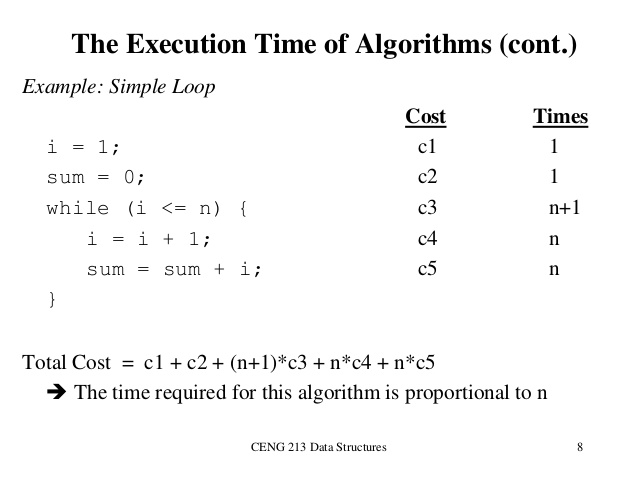
\includegraphics[width=13cm]{aa.jpg}
        \justify
        Esta interpolación me interesa porque con estos acercamientos rigurosos a lo que coloquialmente consideramos un conjunto de pasos ordenados, nos permite crear códigos (y por ende, programas) mas eficientes en sus funciones, permitiendo crear estándares de industria.
        \section{Conclusión}
        \justify
        Las aplicaciones expuestas muestran que la Investigación de Operaciones se puede aplicar en muchos (si es que todos) los aspectos de la vida en los cuales se necesite una optimización pertinente para un fin. En ambas se muestra la importancia de las computadoras
        y sus sistemas como una herramienta clave y un campo de estudio necesario para contribuir a las disciplinas de Ciencias Computacionales y la Investigación de operaciones.
    \end{justify}

    \newpage
        \lhead{}
        \addcontentsline{toc}{section}{Referencias}
        \printbibliography
\end{document}